\htwo{Middleware}

Eine Middleware ist eine Funktion, welche vor dem Controller aufgerufen wird. Diese nimmt die aus "ExpressJS" bekannten Parameter "Request", "Response" und "Next". Middlewares können sowohl für die gesamte API im App-Konstruktor registriert werden als auch für einzelne Controller, bzw. einzelne Methoden in Controllern.

Eine Middleware könnte zum Beispiel Informationen über die "Requests" loggen. 

\begin{figure}[h]
    \centering
    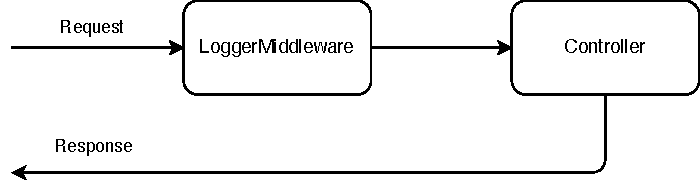
\includegraphics{media/APITemplate/LogMiddleware.svg.pdf}
    \caption{Aufrufreihenfolge Beispiel Log-Middleware} 
\end{figure}

Allerdings können Middlewares auch benutzt werden, um Nutzer auf bestimme Controller zu Autorisieren. Dabei wird in der Middleware geprüft, ob der Nutzer auf diesen "Endpoint" zugreifen darf. Wenn ja, wird die "Next"-Funktion aufgerufen. Wenn nicht, wird eine "Unauthorised-Response" geschickt.

\begin{figure}[h]
    \centering
    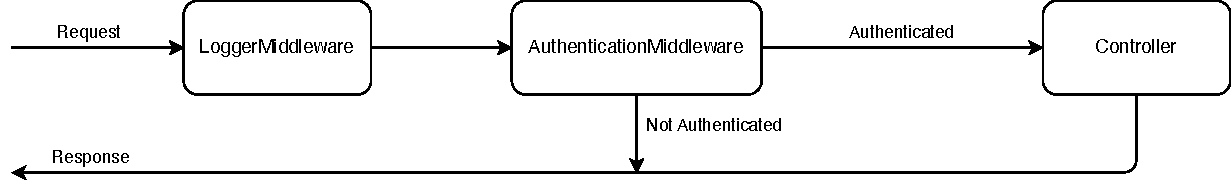
\includegraphics[width=15cm]{media/APITemplate/AuthMiddleware.svg.pdf}
    \caption{Aufrufreihenfolge Beispiel Authentication-Middleware} 
\end{figure}